\documentclass[10pt,pdf,utf8,russian,aspectratio=169]{beamer}
\usepackage[T2A]{fontenc}
\usepackage[english,russian]{babel}
\usepackage{cmap}
\usepackage{subfig}
\usepackage{graphicx}
\usepackage{multicol}
\usepackage{cancel}
\usepackage{tabularx}
%
% Choose how your presentation looks.
%
% For more themes, color themes and font themes, see:
% http://deic.uab.es/~iblanes/beamer_gallery/index_by_theme.html
%
\mode<presentation>
{
  \usetheme{Boadilla}      % or try Darmstadt, Madrid, Warsaw, ...
  \usecolortheme{seagull} % or try albatross, beaver, crane, ..

  \usefonttheme{structurebold}  % or try serif, structurebold, ...
  \setbeamertemplate{navigation symbols}{}
  \setbeamertemplate{caption}[numbered]
} 

\captionsetup[subfloat]{labelformat=empty}
\title[Оптимизация гиперпараметров]{Оптимизация гиперпараметров градиентными методами}
\author{Бахтеев Олег}
\institute{МФТИ}
\date{04.04.2018}
%\renewcommand{\headrulewidth}{0pt}
\DeclareMathOperator*{\argmin}{arg\,min}
\DeclareMathOperator*{\argmax}{arg\,max}
\begin{document}

\begin{frame}
  \titlepage
\end{frame}



\begin{frame}{Градиентные методы: зачем?}
\begin{columns}
\begin{column}{0.5\textwidth}
\begin{itemize}
\item Гиперпараметры --- параметры распределения параметров модели.
\item Основные методы оптимизации не позволяют проводить оптимизацию большого количества гиперпараметров (>10).
\item Решение проблемы --- использование градиентного спуска для гиперпараметров.
\end{itemize}
\end{column}
\begin{column}{0.4\textwidth}
\begin{figure}[h]
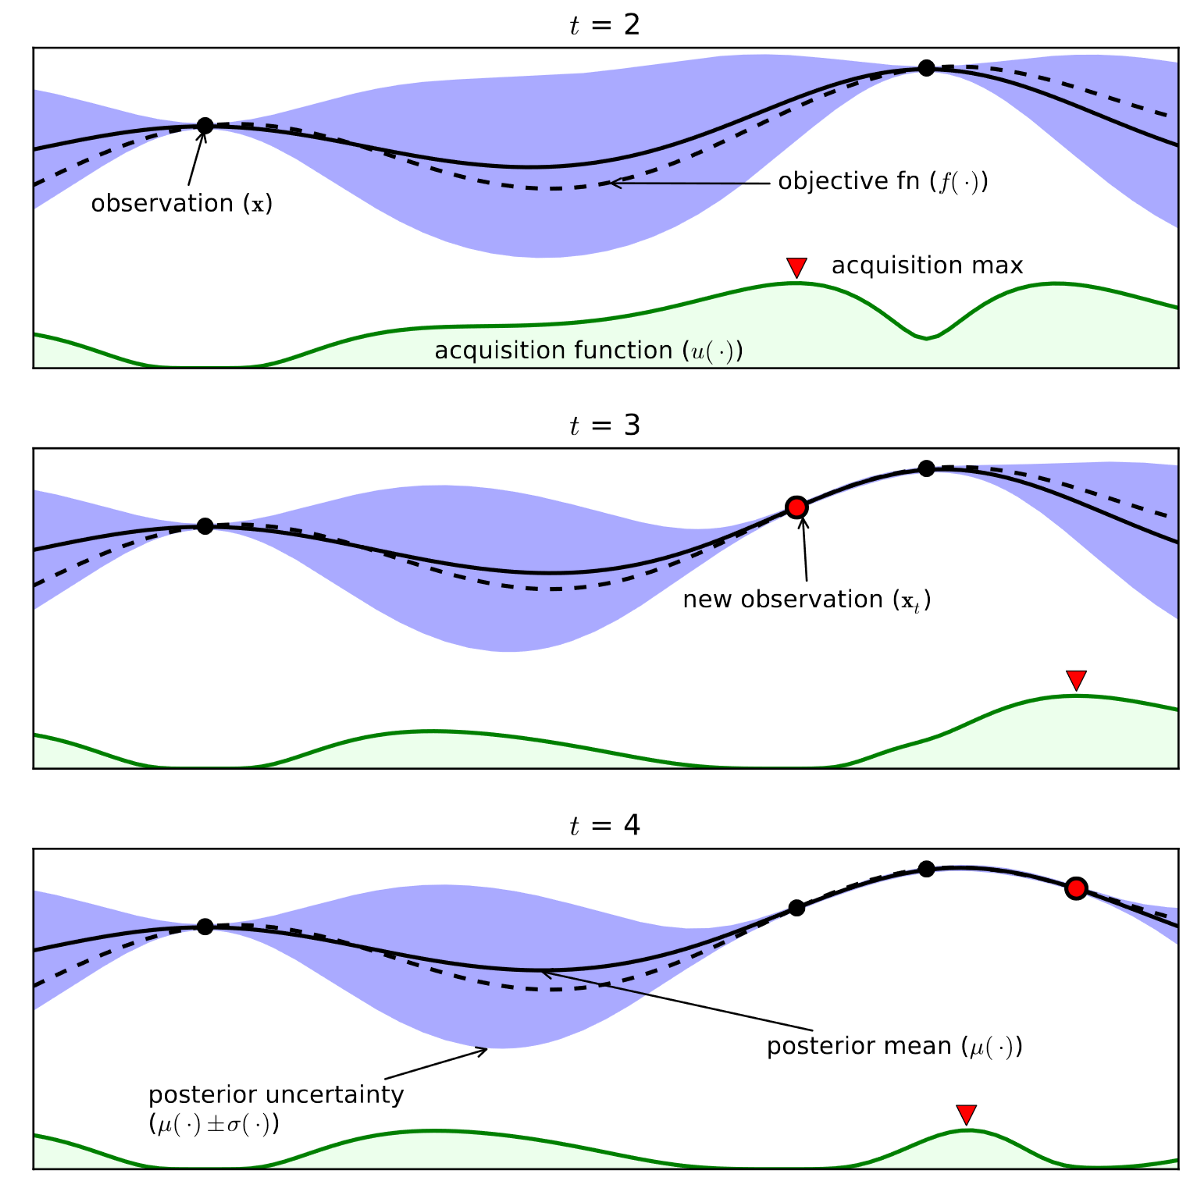
\includegraphics[width=\textwidth]{./gp.png}
\caption*{Shahriari et. al, 2016. Пример работы гауссового процесса.}
\end{figure}

\end{column}
\end{columns}

\end{frame}



\begin{frame}{Постановка задачи}
Задана дифференцируемая по параметрам модель, приближающая зависимую переменную~$y$:
\[
	f:\mathbb{R}^n \to \mathbb{Y}, \quad \mathbf{w} \in \mathbb{R}^u.
\]
Функция $f$ задает правдоподобие выборки $\text{log}p(\mathbf{y}|\mathbf{X}, f)$. 

Пусть также задано априорное распределение параметров: $$\mathbf{w} \sim \mathcal{N}(\mathbf{0}, \mathbf{A}^{-1}),$$
где $\mathbf{A}^{-1} = \text{diag}[\alpha_1, \dots, \alpha_u]^{-1}$ --- матрица ковариаций диагонального вида, определяемая \textit{гиперпараметрами} $[\alpha_1, \dots, \alpha_u]$.
\end{frame}
\begin{frame}{Кросс-валидация}
Разобьем выборку $\mathfrak{D}$ на $k$ равных частей:
\[
\mathfrak{D} = \mathfrak{D}_1 \sqcup \dots \sqcup \mathfrak{D}_k.
\]


Запустим $k$ оптимизаций модели, каждую на своей части выборки. Положим $\boldsymbol{\theta} = [\mathbf{w}_1, \dots, \mathbf{w}_k]$, где $\mathbf{w}_1, \dots, \mathbf{w}_k$ --- параметры модели при оптимизации $k$.
 
Пусть $L$ --- функция потерь:
\begin{equation}
\label{eq:cv}
L(\boldsymbol{\theta}, \mathbf{A}^{-1}) = -\frac{1}{k}\sum_{q=1}^k \bigl(\frac{k}{k-1}\text{log}p(\mathbf{y} \setminus \mathbf{y}_q|\mathbf{X}\setminus \mathbf{X}_q, \mathbf{w}_q) + \text{log}p(\mathbf{w}_q|\mathbf{A})\bigr).
\end{equation}

Пусть $Q$ --- функция качества модели:
\[
Q(\boldsymbol{\theta}, \mathbf{A}^{-1}) = \frac{1}{k}\sum_{q=1}^k k\text{log}p(\mathbf{y}_q|\mathbf{X}_q, \mathbf{w}_q).
\]

\end{frame}


\begin{frame}{Формальная постановка задачи}
Задана дифференцируемая по параметрам модель, приближающая зависимую переменную~$y$:
\[
	f:\mathbb{R}^n \to \mathbb{Y}, \quad \mathbf{w} \in \mathbb{R}^u.
\]

Пусть $\boldsymbol{\theta} \in \mathbb{R}^s$ --- множество всех оптимизируемых параметров.\\
$L(\boldsymbol{\theta}, \mathbf{A}^{-1})$ ---  дифференцируемая функция потерь  по которой производится оптимизация функции ${f}$. \\
$Q(\boldsymbol{\theta}, \mathbf{A}^{-1})$ ---  дифференцируемая функция определяющая итоговое качество модели ${f}$ и приближающая интеграл.\\

Требуется найти параметры $\hat{\boldsymbol{\theta}}$ и гиперпараметры $\hat{\mathbf{A}}^{-1}$ модели, доставляющие минимум следующему функционалу:
\[
\hat{\mathbf{A}}^{-1} = \argmax_{\mathbf{A}^{-1} \in \mathbb{R}^h} Q(\hat{\boldsymbol{\theta}}(\mathbf{A}^{-1}), \mathbf{A}^{-1}),
\]
\[
	\hat{\boldsymbol{\theta}}(\mathbf{A}^{-1}) =  \argmin_{\boldsymbol{\theta} \in \mathbb{R}^s} L(\boldsymbol{\theta}, \mathbf{A}^{-1}).
\]
\end{frame}
\iffalse
\begin{frame}{Байесовский вывод}
\textit{Первый уровень:}
\[
\hat{\boldsymbol{\theta}} = \argmax \bigl(-L(\boldsymbol{\theta}, \mathbf{A}^{-1})\bigr) = p(\mathbf{w}|\mathbf{X}, \mathbf{y}, \mathbf{A}) = \frac{p(\mathbf{y}|\mathbf{X},\mathbf{w})p(\mathbf{w}|\mathbf{A})}{p(\mathbf{y}|\mathbf{X},\mathbf{A})}.
\]
\textit{Второй уровень:}
\[
p(\mathbf{A}|\mathbf{X}, \mathbf{y}) \propto p(\mathbf{y}|\mathbf{X},\mathbf{A})p(\mathbf{A}),
\]

Полагая распределение параметров $p(\mathbf{A})$ равномерным на некоторой большой окрестности, получим задачу оптимизации гиперпараметров:
\begin{equation}
\label{eq:bayes2}
	Q(\boldsymbol{\theta}, \mathbf{A}^{-1}) = p(\mathbf{y}|\mathbf{X},\mathbf{A}) = \int_{\mathbf{w} \in \mathbb{R}^u} p(\mathbf{y}|\mathbf{X}, \mathbf{w}) p(\mathbf{w}|\mathbf{A}) \to \max_{[\alpha_1, \dots, \alpha_u] \in \mathbb{R}^{n}}.
\end{equation}
\end{frame}
\fi

\begin{frame}{Байесовский подход к сложности}
Правдоподобие модели (``Evidence''):
\[
	p(\mathbf{y}|\mathbf{f}) = \int_\mathbf{w} p(\mathbf{y}|\mathbf{X},\mathbf{w})p(\mathbf{w}|\mathbf{A}) d\mathbf{w}.
\]


\begin{figure}
  \centering
  \subfloat[Схема выбора модели по правдоподобию]{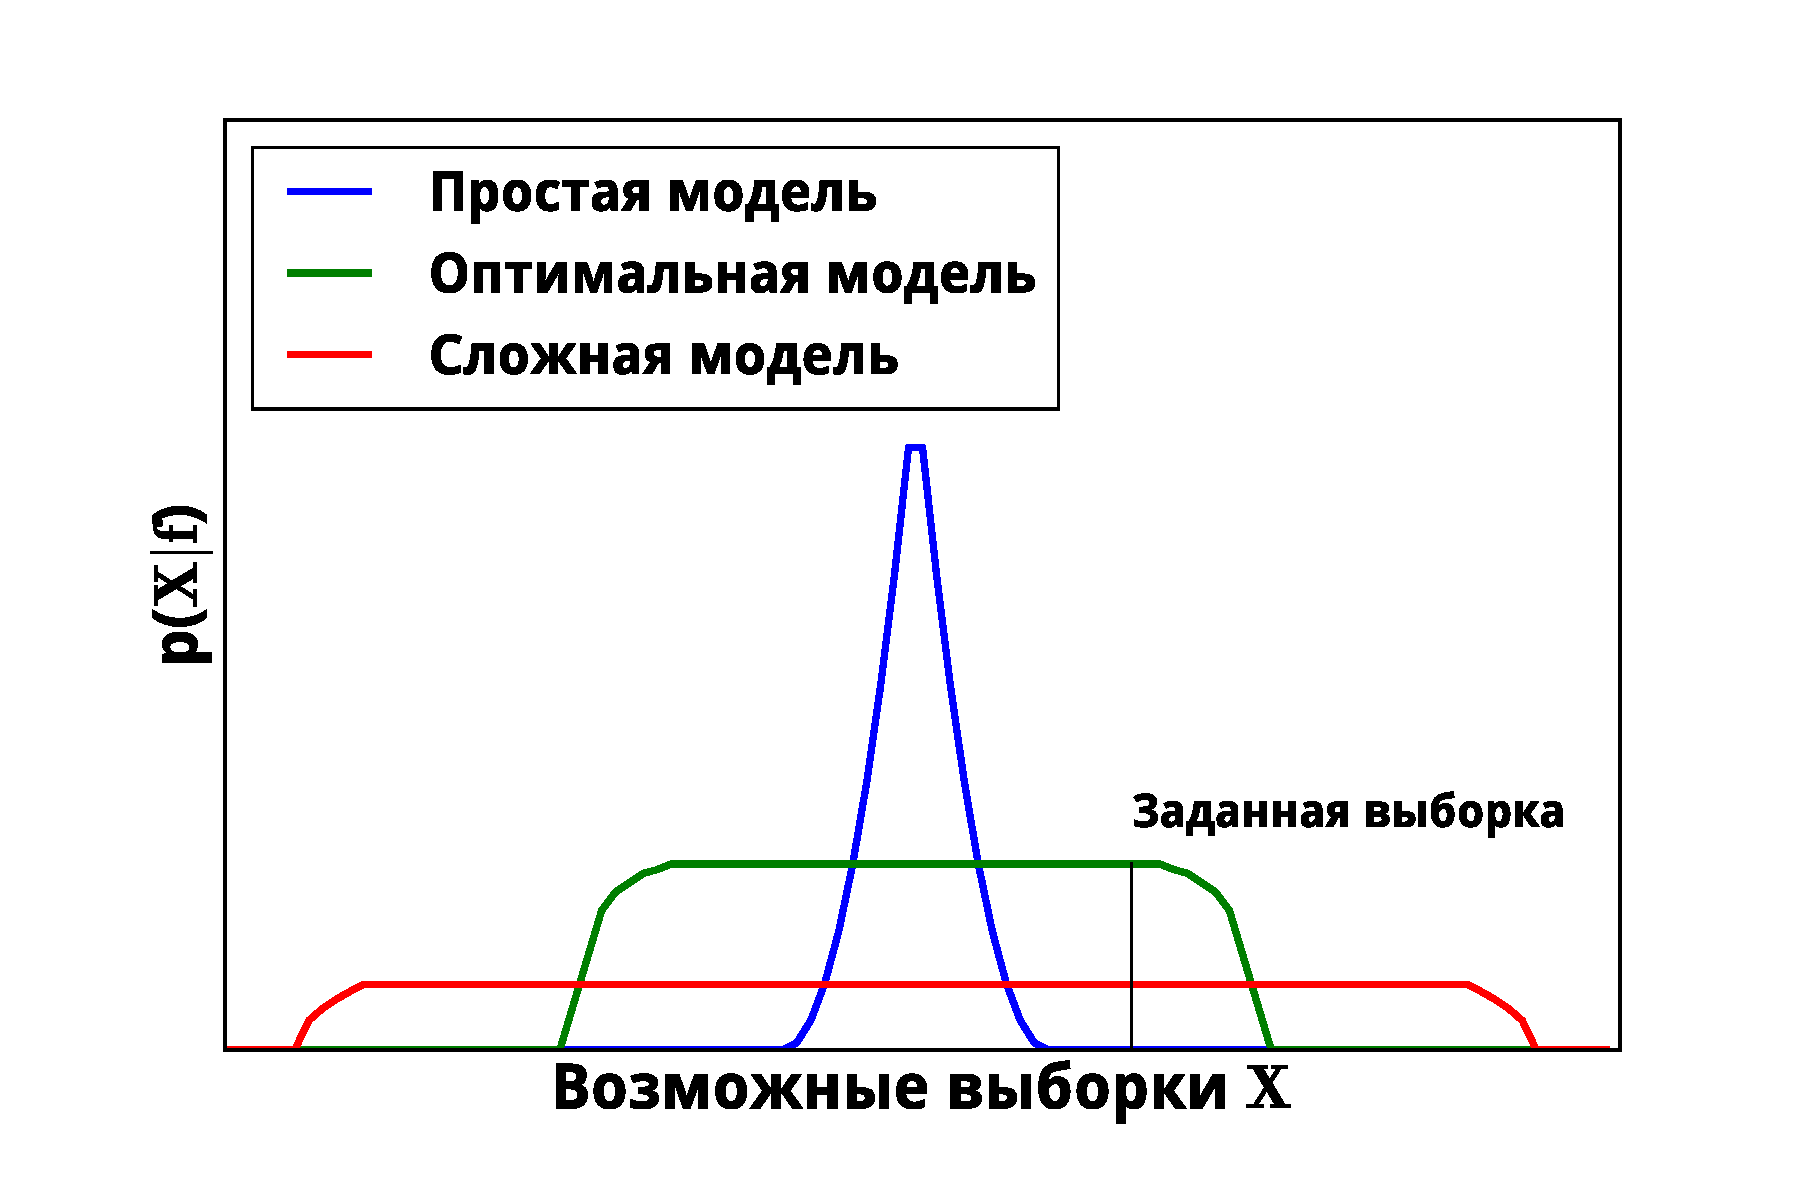
\includegraphics[width=0.4\textwidth]{evidence.pdf}} 
 \subfloat[Пример: полиномы]{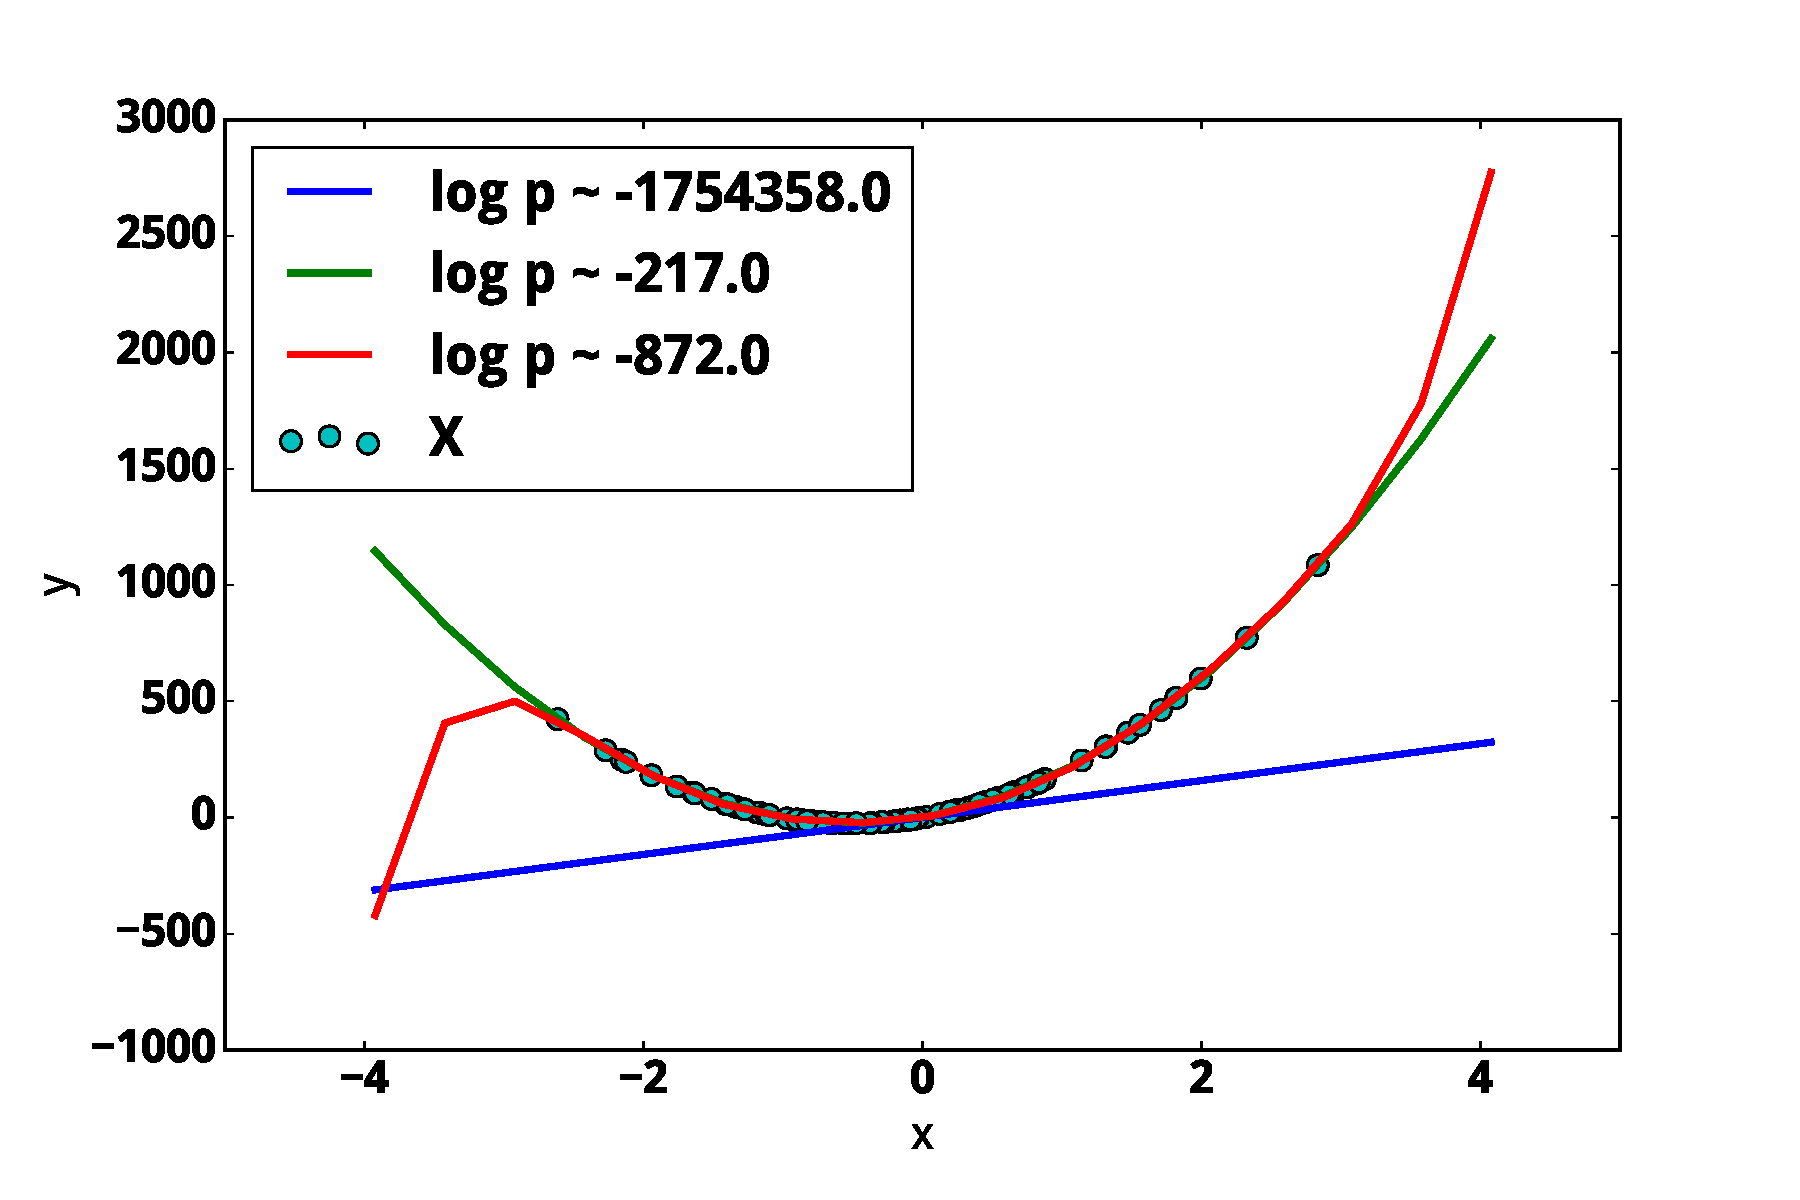
\includegraphics[width=0.4\textwidth]{example.pdf}}
\label{fig:1}\qquad

\end{figure}


\end{frame}


\begin{frame}{Вариационная нижняя оценка}
Пусть задано непрерывное распределение $q$. 
Тогда 
$$
\text{log}~p(\mathbf{y}|\mathbf{X},\mathbf{w})  = \int_{\mathbf{w}} q(\mathbf{w})\text{log}~\frac{p(\mathbf{y},\mathbf{w}|\mathbf{X},\mathbf{A})}{q(\mathbf{w})}d\mathbf{w} + \text{D}_\text{KL}  (q(\mathbf{w})||p(\mathbf{w}| \mathbf{y}, \mathbf{X}, \mathbf{A})) \geq	
$$
$$
\geq \int_{\mathbf{w}} q(\mathbf{w})\text{log}~\frac{p(\mathbf{y},  \mathbf{w}|\mathbf{X}, \mathbf{A})}{q(\mathbf{w})}d\mathbf{w} =
$$

$$
= -\text{D}_\text{KL} (q(\mathbf{w})||p(\mathbf{w}|\mathbf{A})) + \int_{\mathbf{w}} q(\mathbf{w})\text{log}~{p(\mathbf{y}|\mathbf{X}, \mathbf{w},\mathbf{A})} d \mathbf{w},
$$
где $$\text{D}_\text{KL}(q(\mathbf{w})||p(\mathbf{w} |\mathbf{A})) = -\int_{\mathbf{w}} q(\mathbf{w})\text{log}~\frac{p(\mathbf{w} | \mathbf{A})}{q(\mathbf{w})}d\mathbf{w}.$$

\end{frame}


\begin{frame}{Evidence: нормальное распределение}
\textbf{``Обычная'' функция потерь:}\\
$$
L = \textcolor{red}{\sum_{\mathbf{x}, \mathbf{y} \in \mathfrak{D}} - \text{log}p(\mathbf{y}|\mathbf{x}, \mathbf{w})} + \textcolor{blue}{\lambda||\mathbf{w}||_2^2}.
$$\\~\\

% если n - константна.
\textbf{Вариационный вывод при $p(\mathbf{w}|\mathbf{f}) \sim \mathcal{N}(\mathbf{0}, \mathbf{1})$:}\\
$$
L =   \textcolor{red}{\sum_{\mathbf{x}, \mathbf{y} \in \mathfrak{D}} \text{log}~p(\mathbf{y}|\mathbf{x}, \hat{\mathbf{w}})} +
 \textcolor{blue}{\frac{1}{2} \bigl( \text{tr} (\mathbf{A}^{-1}_q) + \boldsymbol{\mu}_q^\text{T}\mathbf{A}\boldsymbol{\mu}_q  - \text{ln}~|\mathbf{A}^{-1}_q| \bigr)},
$$\\$$\hat{\mathbf{w}} \sim q = \mathcal{N}(\boldsymbol{\mu}_q, \mathbf{A}^{-1}_q).$$~\\


\end{frame}

\begin{frame}{Вариационная оценка: оптимизация гиперпараметров}
Пусть $L=-Q$:
\[
\label{eq:elbo}
\text{log}~p(\mathbf{y}|\mathbf{X},\mathbf{A})  
\geq 
\sum_{\mathbf{x},y} \text{log}~p({y}|\mathbf{x}, \hat{\mathbf{w}}) - D_\text{KL}\bigl(q (\mathbf{w}) || p (\mathbf{w}|\mathbf{A})\bigr) = -L(\boldsymbol{\theta}, \mathbf{A}^{-1}) = Q(\boldsymbol{\theta}, \mathbf{A}^{-1}),
\]
где $q$ --- нормальное распределение с диагональной матрицей ковариаций:
\[
\label{eq:diag}
	q \sim \mathcal{N}(\boldsymbol{\mu}_q, \mathbf{A}^{-1}_q),
\]
$$
D_\text{KL}\bigl(q (\mathbf{w}) || p (\mathbf{w}|\mathbf{f})\bigr) = \frac{1}{2} \bigl( \text{Tr} [\mathbf{A}\mathbf{A}^{-1}_q] + (\boldsymbol{\mu} - \boldsymbol{\mu}_q)^\mathsf{T}\mathbf{A}(\boldsymbol{\mu} - \boldsymbol{\mu}_q) - u +\text{ln}~|\mathbf{A}^{-1}| - \text{ln}~|\mathbf{A}_q^{-1}| \bigr).
$$

В качестве оптимизируемых параметров $\boldsymbol{\theta}$ выступают параметры распределения $q$:
\[
\boldsymbol{\theta} = [\alpha_1, \dots, \alpha_u, {\mu}_1,\dots,{\mu}_u].
\]


\end{frame}


\begin{frame}{Формальная постановка задачи: градиентная оптимизация}
\begin{block}{Определение}
Оператором $T$ назовем оператор стохастического градиентного спуска, производящий $\eta$ шагов оптимизации:
\begin{equation}
\label{eq:gd}
	 \hat{\boldsymbol{\theta}} = T \circ T \circ \dots \circ T(\boldsymbol{\theta}_0, \mathbf{A}^{-1}) = T^\eta(\boldsymbol{\theta}_0, \mathbf{A}^{-1}),
\end{equation}
где 
$$
	T(\boldsymbol{\theta}, \mathbf{A}^{-1}) =\boldsymbol{\theta} - \gamma \nabla L(\boldsymbol{\theta}, \mathbf{A}^{-1})|_{\hat{\mathfrak{D}}}, 
$$
$\gamma$ --- длина шага градиентного спуска, $\boldsymbol{\theta}_0$ --- начальное значение параметров $\boldsymbol{\theta}$, $\hat{\mathfrak{D}}$ --- случайная подвыборка исходной выборки $\mathfrak{D}$.
\end{block}


Перепишем итоговую задачу оптимизации:
\[
	\hat{\mathbf{A}}^{-1} = \argmax_{\mathbf{A}^{-1} \in \mathbb{R}^h} Q( T^\eta(\boldsymbol{\theta}_0, \mathbf{A}^{-1})),
\]
где $\boldsymbol{\theta}_0$ --- начальное значение параметров $\boldsymbol{\theta}$.


\end{frame}


\begin{frame}{RMAD, Maclaurin et. al, 2015 }
\begin{columns}
\begin{column}{0.5\textwidth}
\begin{enumerate}
\item Провести $\eta$ шагов оптимизации: $\boldsymbol{\theta} = T(\boldsymbol{\theta}_0, \mathbf{A}^{-1})$.
\item Положим $\hat{\nabla} \mathbf{A}^{-1} = \nabla_\mathbf{A}^{-1} Q(\boldsymbol{\theta}, \mathbf{A}^{-1}).$ 
\item Положим $d\mathbf{v} = \mathbf{0}.$
\item Для $\tau = \eta \dots 1 $ повторить:
\item $\boldsymbol{\theta}^{\tau-1} =  \boldsymbol{\theta}^{\tau} - \gamma\mathbf{v}^{\tau}.$
\item $\mathbf{v}^{\tau-1} =\mathbf{v}^{\tau} + \gamma \hat{\nabla}_{\boldsymbol{\theta}}.$
\item $d\mathbf{v} =  \gamma \hat{\nabla}_{\boldsymbol{\theta}}$.
\item $\hat{\nabla} \mathbf{A}^{-1} =  \hat{\nabla} \mathbf{A}^{-1} - d\mathbf{v}\nabla_{\mathbf{A}^{-1}} \nabla_{\boldsymbol{\theta}} Q$.
\item $\hat{\nabla} \boldsymbol{\theta}  = \hat{\nabla} \boldsymbol{\theta}  - d\mathbf{v}\nabla_{\boldsymbol{\theta}} \nabla_{\boldsymbol{\theta}} Q$.
\end{enumerate}
\end{column}

\begin{column}{0.5\textwidth}
Алгоритм RMAD основывается на Reverse-mode differentiation.
\begin{figure}
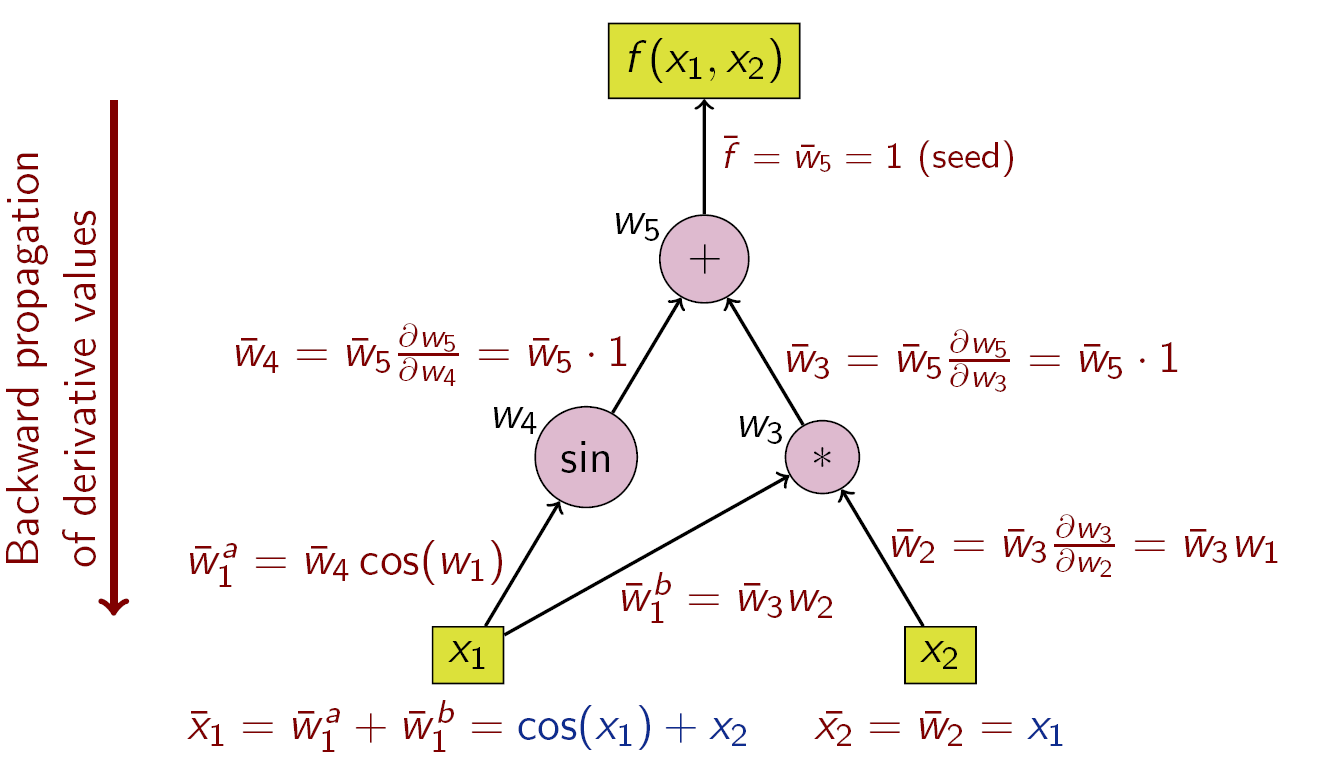
\includegraphics[width=\textwidth]{rmd.png}
\end{figure}
\end{column}
\end{columns}
\end{frame}


\begin{frame}{DrMAD}
Алгоритм DrMad --- упрощенный RMAD. 
Вводится предположение о линейности траектории обновления параметров $\boldsymbol{\theta}$.
\begin{columns}
\begin{column}{0.5\textwidth}
\begin{enumerate}
\item Провести $\eta$ шагов оптимизации: $\boldsymbol{\theta} = T(\boldsymbol{\theta}_0, \mathbf{A}^{-1})$.
\item Положим $\hat{\nabla} \mathbf{A}^{-1} = \nabla_\mathbf{A}^{-1} Q(\boldsymbol{\theta}, \mathbf{A}^{-1}).$ 
\item Положим $d\mathbf{v} = \mathbf{0}.$
\item Для $\tau = \eta \dots 1 $ повторить:
\item $\boldsymbol{\theta}^{\tau-1} =  \boldsymbol{\theta}^{\tau} - \gamma\mathbf{v}^{\tau}.$
\item $\mathbf{v}^{\tau-1} =\mathbf{v}^{\tau} + \gamma \hat{\nabla}_{\boldsymbol{\theta}}.$
\item $d\mathbf{v} =  \gamma \hat{\nabla}_{\boldsymbol{\theta}}$.
\item $\hat{\nabla} \mathbf{A}^{-1} =  \hat{\nabla} \mathbf{A}^{-1} - d\mathbf{v}\nabla_{\mathbf{A}^{-1}} \nabla_{\boldsymbol{\theta}} Q$.
\item $\hat{\nabla} \boldsymbol{\theta}  = \hat{\nabla} \boldsymbol{\theta}  - d\mathbf{v}\nabla_{\boldsymbol{\theta}} \nabla_{\boldsymbol{\theta}} Q$.
\end{enumerate}
\end{column}
\begin{column}{0.5\textwidth}
\begin{enumerate}
\item Провести $\eta$ шагов оптимизации: $\boldsymbol{\theta} = T(\boldsymbol{\theta}_0, \mathbf{A}^{-1})$.
\item Положим $\hat{\nabla} \mathbf{A}^{-1} = \nabla_\mathbf{A}^{-1} Q(\boldsymbol{\theta}, \mathbf{A}^{-1}).$ 
\item Положим $d\mathbf{v} = \mathbf{0}.$
\item Для $\tau = \eta \dots 1 $ повторить:
\item $\boldsymbol{\theta}^{\tau-1} = \boldsymbol{\theta}_0 + \frac{\tau-1}{\eta} \boldsymbol{\theta}^{\eta}.$
\item ~
\item $d\mathbf{v} =  \gamma \hat{\nabla}_{\boldsymbol{\theta}}$.
\item $\hat{\nabla} \mathbf{A}^{-1} =  \hat{\nabla} \mathbf{A}^{-1} - d\mathbf{v}\nabla_{\mathbf{A}^{-1}} \nabla_{\boldsymbol{\theta}} Q$.
\item $\hat{\nabla} \boldsymbol{\theta}  = \hat{\nabla} \boldsymbol{\theta}  - d\mathbf{v}\nabla_{\boldsymbol{\theta}} \nabla_{\boldsymbol{\theta}} Q$.
\end{enumerate}
\end{column}
\end{columns}
\end{frame}



\begin{frame}{Аналитическая формула оптимизации параметров}
\textbf{Утверждение (Pedregosa, 2016).}\\
Пусть $L$ --- дифференцируемая функция, такая что все стационарные точки $L$ являются локальными минимумами.
Пусть также гессиан $\mathbf{H}^{-1}$ функции потерь $L$ является обратимым в каждой стационарной точке.\\
Тогда
\[
\nabla_{\mathbf{A}^{-1}}Q(T(\boldsymbol{\theta}_0), \mathbf{A}^{-1}) =  \nabla_{\mathbf{A}^{-1}}Q(\boldsymbol{\theta}^\eta, \mathbf{A}^{-1}) - \nabla_{\mathbf{A}^{-1}}\nabla_{\boldsymbol{\theta}} L(\boldsymbol{\theta}^\eta, \mathbf{A}^{-1})^\text{T}\mathbf{H}^{-1}\nabla_{\boldsymbol{\theta}}Q(\boldsymbol{\theta}^\eta, \mathbf{A}^{-1}).
\]

\textbf{Схема доказательства}\\
\begin{enumerate}
\item Т.к. точка $\boldsymbol{\theta}^\eta$ стационарна, то $\nabla_{\boldsymbol{\theta}} L(\boldsymbol{\theta}^\eta, \mathbf{A}^{-1}) = 0$.
\item Продифференцируем выражение по $\mathbf{A}^{-1}:$
\[
    \nabla_{\mathbf{A}^{-1}}\nabla_{\boldsymbol{\theta}} L(\boldsymbol{\theta}^\eta, \mathbf{A}^{-1} + \mathbf{A}^{-1}\nabla_{\mathbf{A}^{-1}}T(\boldsymbol{\theta}_0).
\]
\item По правилу дифференцирования сложной функции:
\[
\nabla_{\mathbf{A}^{-1}}Q(T(\boldsymbol{\theta}_0), \mathbf{A}^{-1}) =  \nabla_{\mathbf{A}^{-1}}Q(\boldsymbol{\theta}^\eta, \mathbf{A}^{-1})  + \nabla_{\mathbf{A}^{-1}}T(\boldsymbol{\theta}_0)^\text{T}\nabla_{\boldsymbol{\theta}}Q(\boldsymbol{\theta}^\eta, \mathbf{A}^{-1}).
\]
\item Подставим в выражение 3 выражение 2 и получим искомое.
\end{enumerate}
\end{frame}


\begin{frame}{Жадная оптимизация гиперпараметров}
На каждом шаге оптимизации параметров $\boldsymbol{\theta}$:
\[
	\mathbf{A}'^{-1} = \mathbf{A}^{-1} - \gamma_{\mathbf{A}^{-1}} \nabla_{\mathbf{A}^{-1}}  Q \bigl(T(\boldsymbol{\theta}, \mathbf{A}^{-1}) , \mathbf{A}^{-1}\bigr) = \mathbf{A}^{-1} - \gamma_{\mathbf{A}^{-1}} \nabla_{\mathbf{A}^{-1}}  Q\bigl(\boldsymbol{\theta} - \gamma \nabla L(\boldsymbol{\theta}, \mathbf{A}^{-1}), \mathbf{A}^{-1})\bigr),
\]
где $\gamma_{\mathbf{A}^{-1}}$ --- длина шага оптимизации гиперпараметров.

\begin{itemize}
\item Можно рассматривать как упрощение алгоритма RMAD, использующее только один элемент истории обновления параметров.
\item Является приближением к решению аналитической формуле в случае $\mathbf{H}^{-1} \sim \mathbf{I}$.
\end{itemize}

\end{frame}


\begin{frame}{HOAG}
Численное приближение аналитической формулы:
 \[\nabla_{\mathbf{A}^{-1}}Q(\boldsymbol{\theta}^\eta, \mathbf{A}^{-1}) - \nabla_{\mathbf{A}^{-1}}\nabla_{\boldsymbol{\theta}} L(\boldsymbol{\theta}^\eta, \mathbf{A}^{-1})^\text{T}\mathbf{H}^{-1}\nabla_{\boldsymbol{\theta}}Q(\boldsymbol{\theta}^\eta, \mathbf{A}^{-1}).\]
\begin{enumerate}
\item Провести $\eta$ шагов оптимизации: $\boldsymbol{\theta} = T(\boldsymbol{\theta}_0, \mathbf{A}^{-1})$.
\item Решить линейную систему для вектора $\boldsymbol{\lambda}$: $\mathbf{H}^{-1}(\boldsymbol{\theta})\boldsymbol{\lambda} =  \nabla_{\boldsymbol{\theta}} Q(\boldsymbol{\theta}, \mathbf{A}^{-1})$.
\item Приближенное значение градиентов гиперпараметра вычисляется как: $\hat{\nabla}_{\mathbf{A}^{-1}}Q = \nabla_{\mathbf{A}^{-1}}Q(\boldsymbol{\theta}, \mathbf{A}^{-1}) -\nabla_{\boldsymbol{\theta}, \mathbf{A}^{-1}} L(\boldsymbol{\theta}, \mathbf{A}^{-1})^T\boldsymbol{\lambda}$.
\end{enumerate}

Итоговое правило обновления:
\[
\label{eq:update_hyper}
\mathbf{A}'^{-1} = \mathbf{A}^{-1} - \gamma_{\mathbf{A}^{-1}} \hat{\nabla}_{\mathbf{A}^{-1}}Q.
\]


\end{frame}

\begin{frame}{Сравнение алгоритмов}
\begin{table}
%\footnotesize
% Алгоритм & Тип алгоритм & Время & Плюсы & Минусы 

\begin{tabularx}{\textwidth}{|p{2cm}|X|X|}
\hline
\bf Алгоритм &  \bf + & \bf -  \\ \hline
Random search & Легко реализовать & Проклятие размерности  \\ \hline
Жадная оптимизация & Оптимизация проводится внутри цикла оптимизации параметров. Легко реализовать & Жадность, неоптимальность. \\ \hline
HOAG  & Быстрая сходимость.  & Качество результатов зависит от решения линейного уравнения $\mathbf{H}^{-1}(\boldsymbol{\theta})\boldsymbol{\lambda} =  \nabla_{\boldsymbol{\theta}} Q(\boldsymbol{\theta}, \mathbf{A}^{-1})$.\\ \hline 
DrMAD  & Учитывает особенности оператора оптимизации. Можно использовать для оптимизации мета-параметров.& Неустойчив при больших значениях длины градиентного шага $\gamma_\mathbf{A}^{-1}$. Качество оптимизации зависит от кривизны траектории обновления параметров.\\ \hline
\end{tabularx}


\label{table:algo_descr}

\end{table}
\end{frame}

\begin{frame}
\begin{figure}  
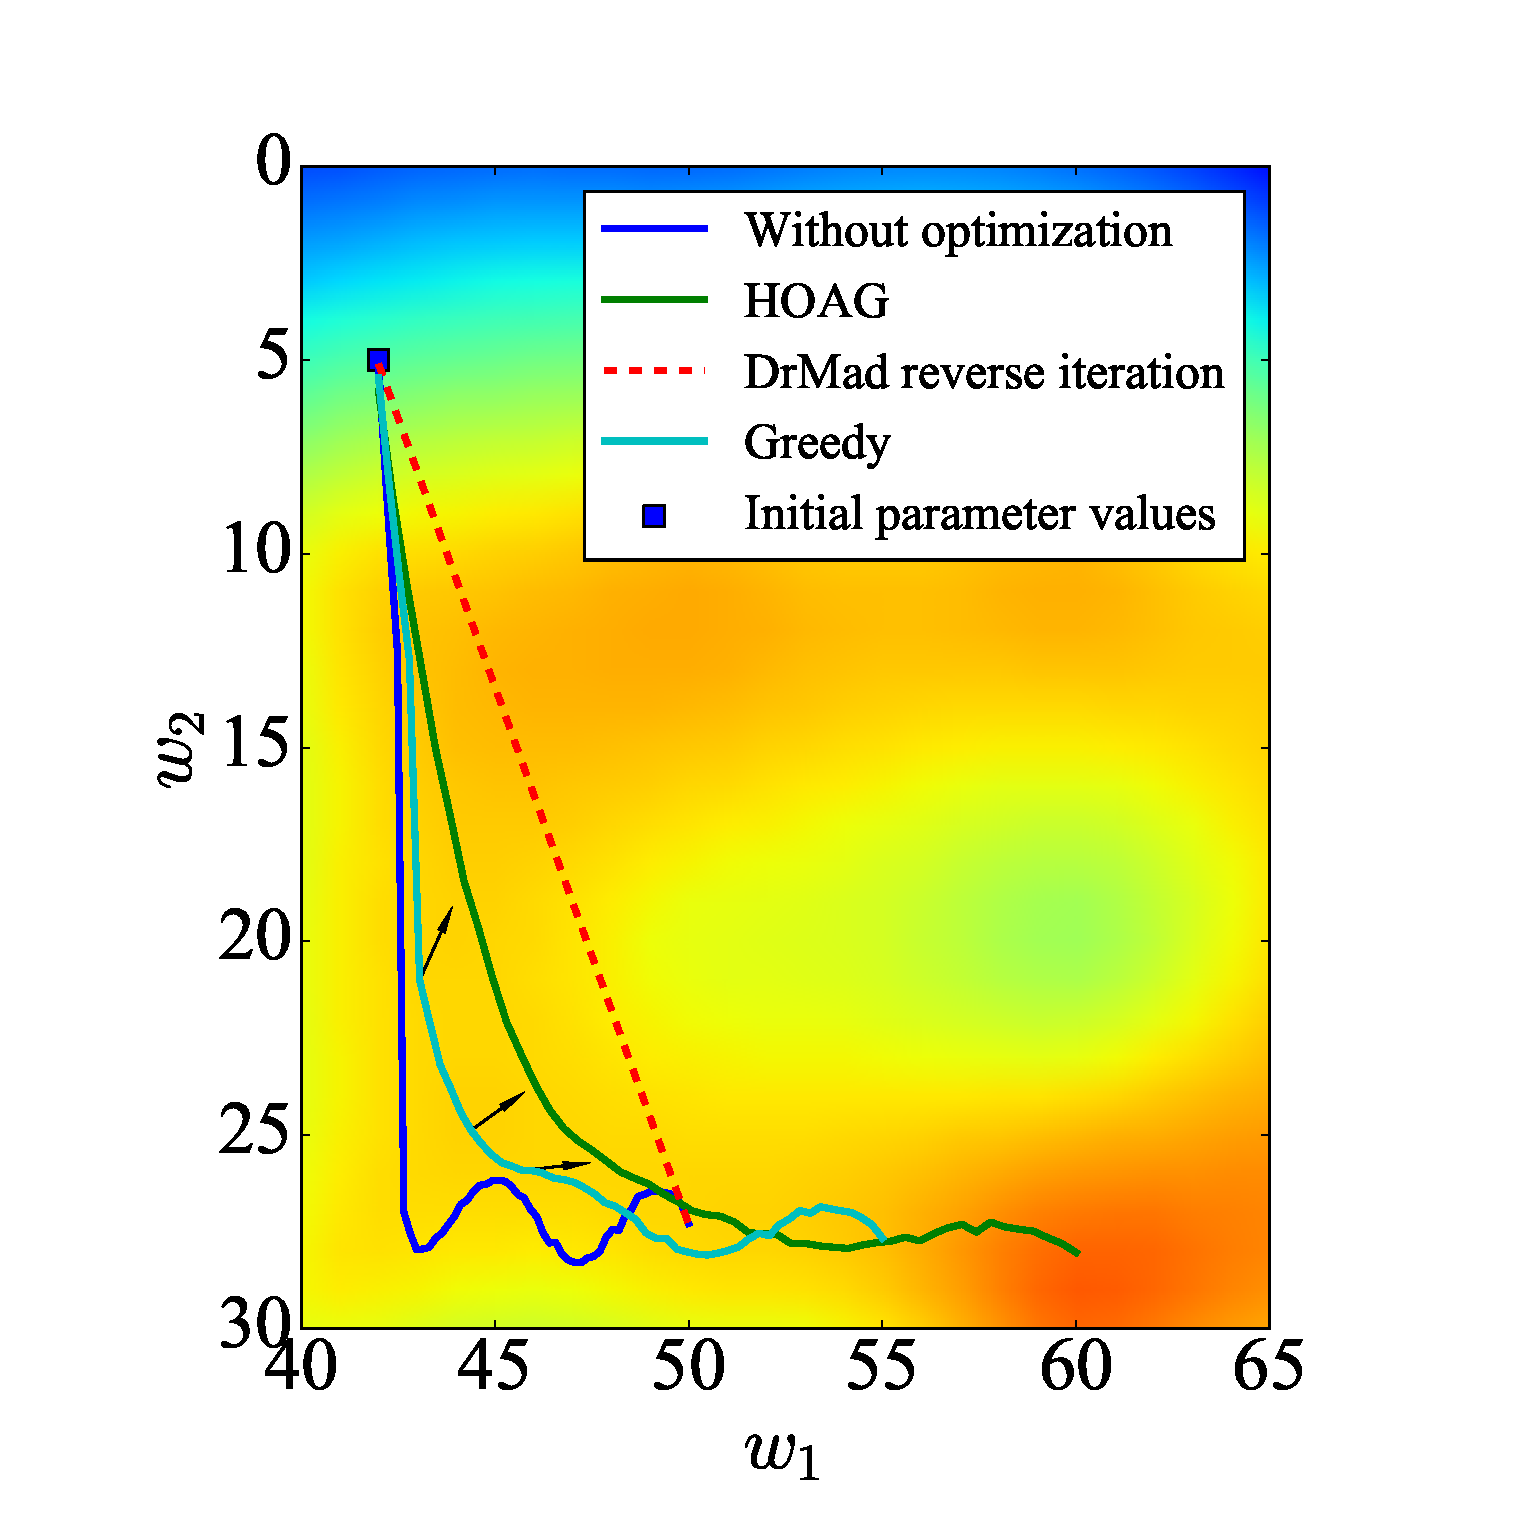
\includegraphics[width=0.5\textwidth]{Fig_traj.eps}
\end{figure}
\end{frame}

\begin{frame}{Эксперименты: полиномы}
\begin{figure}
  \centering
  \subfloat[Кросс-валидация]{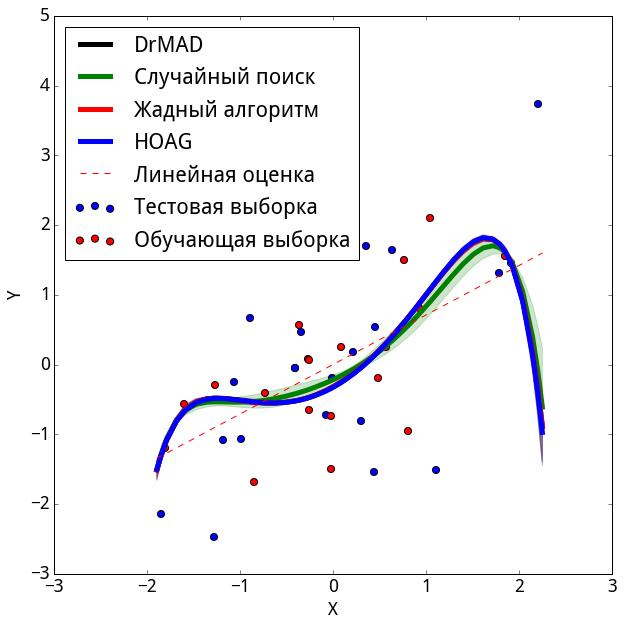
\includegraphics[width=0.42\textwidth]{poly_cv.png}} 
 \subfloat[Evidence]{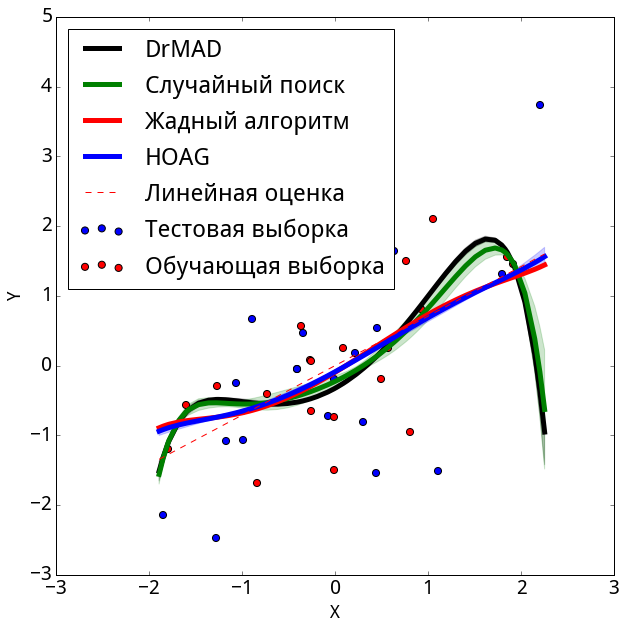
\includegraphics[width=0.42\textwidth]{poly_var.png}}
\label{fig:1}\qquad

\end{figure}
\end{frame}

\begin{frame}{Эксперименты: WISDM}
\begin{figure}  
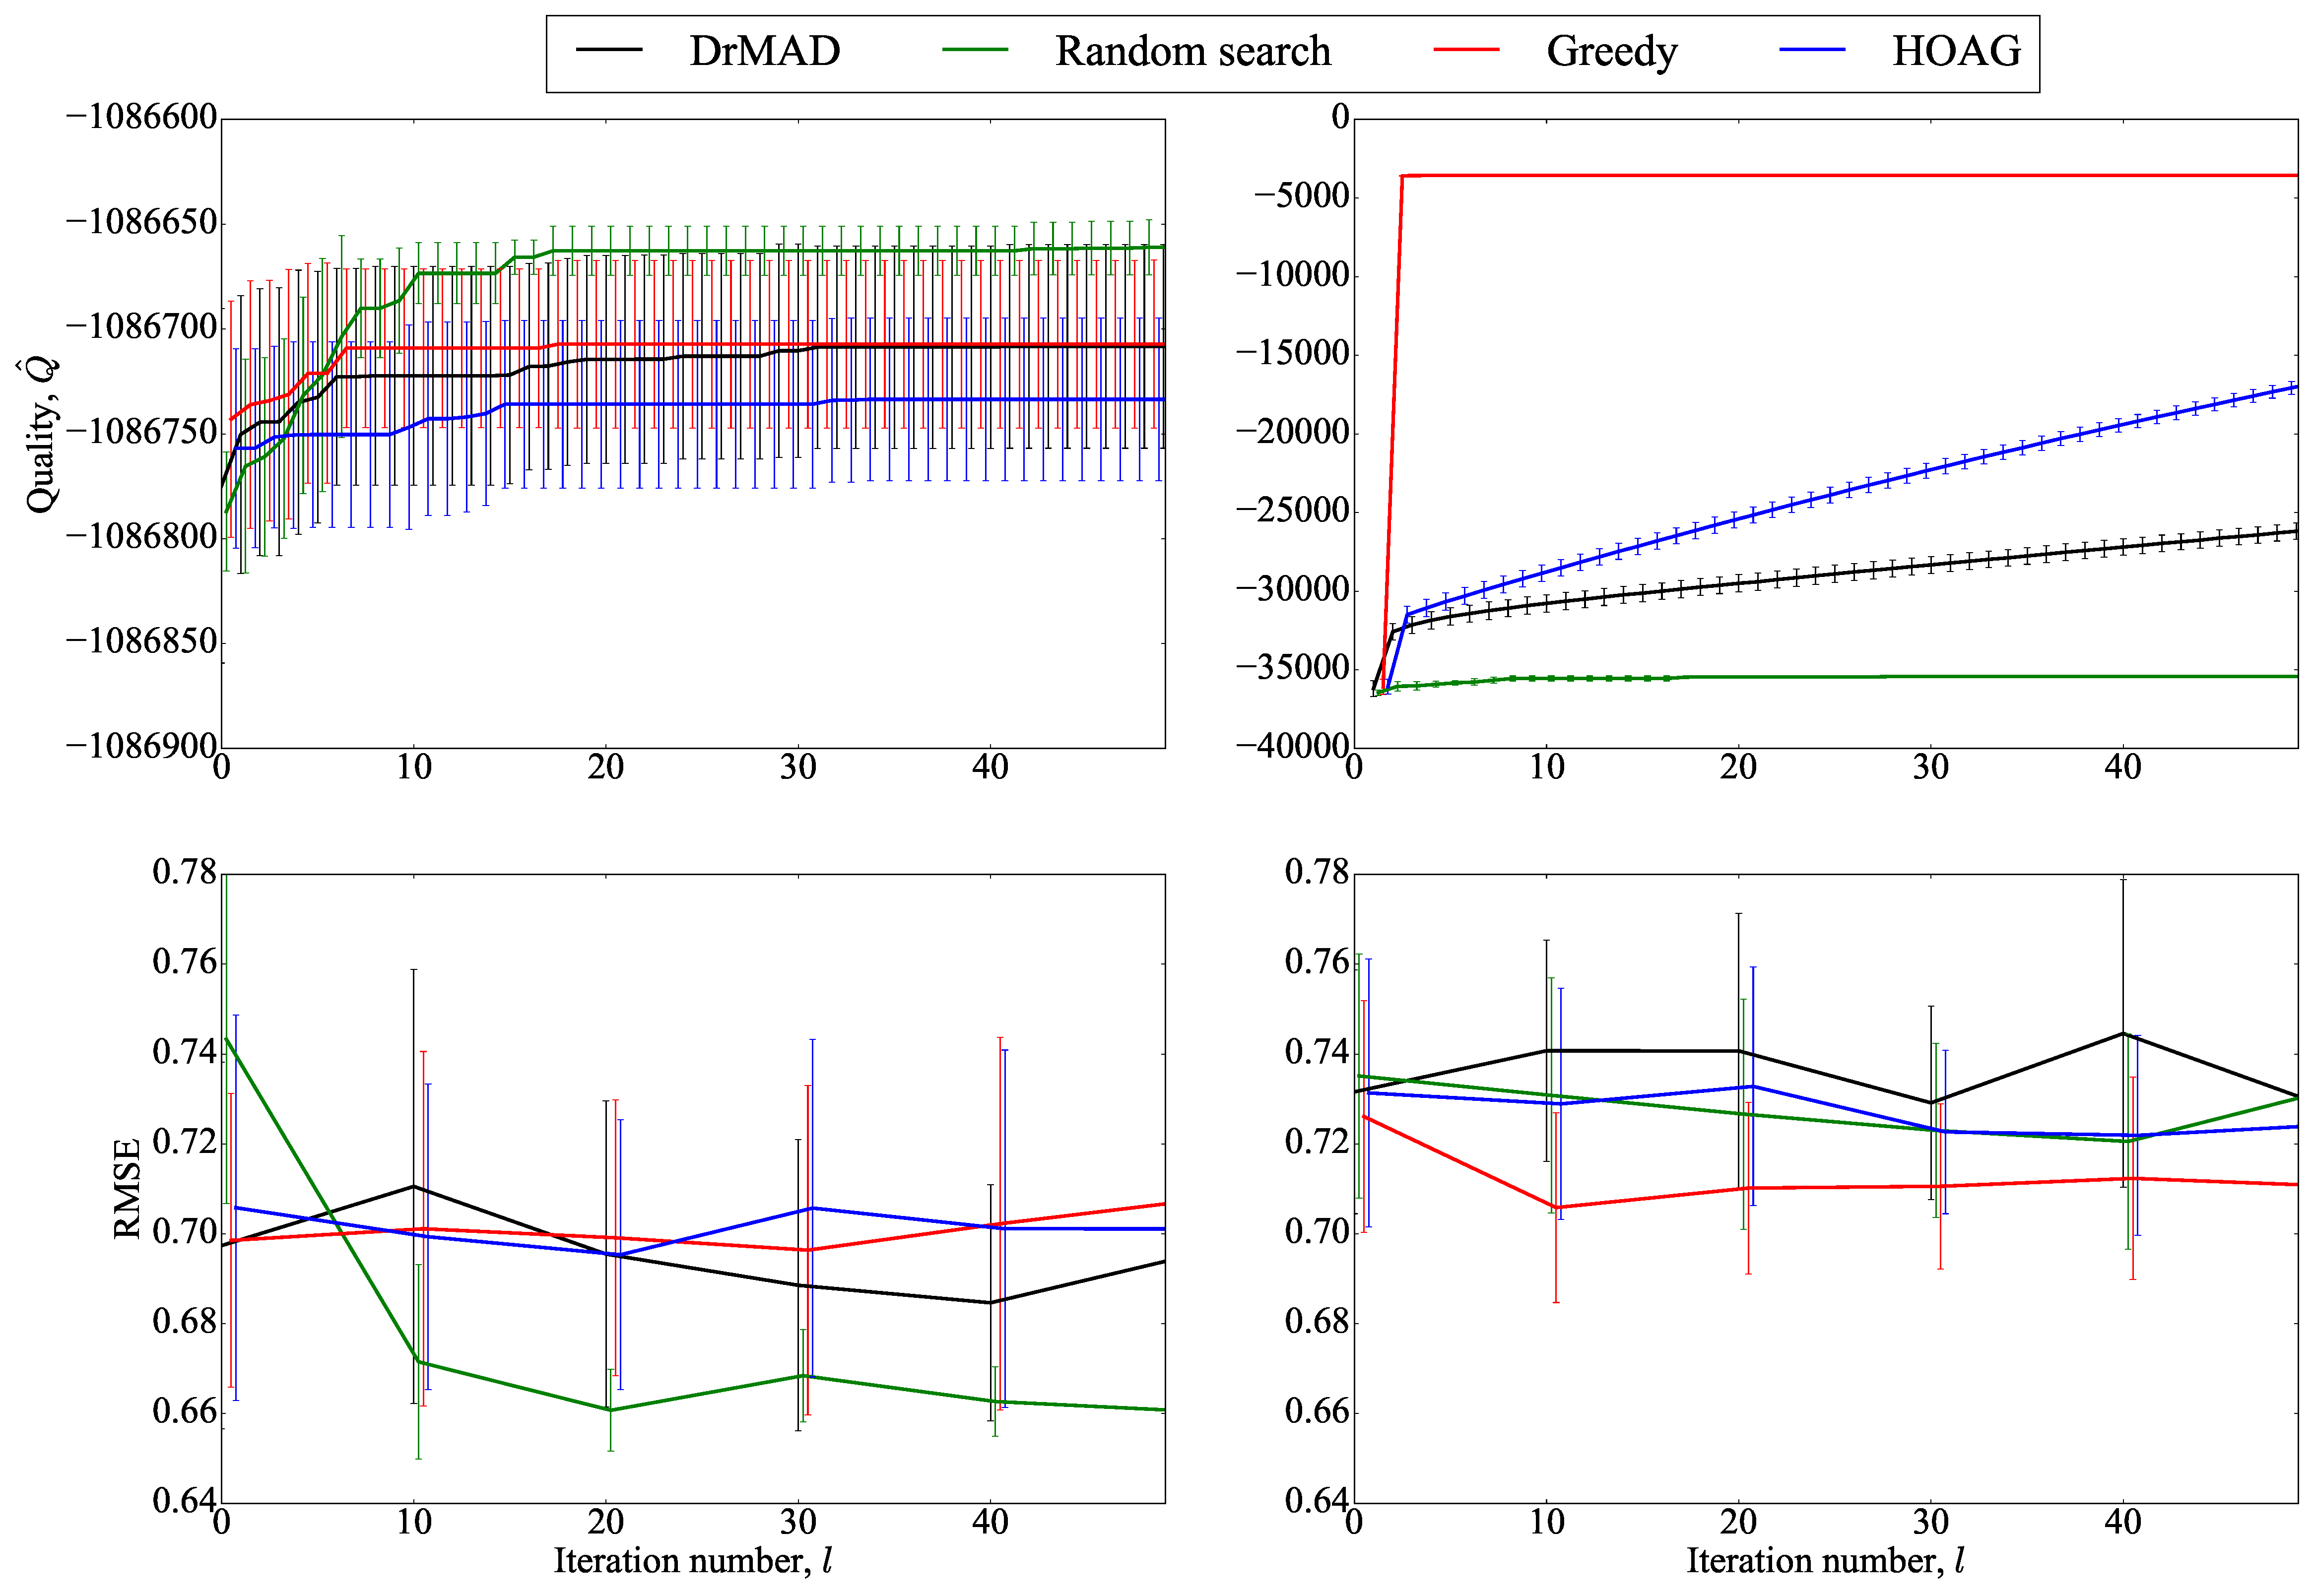
\includegraphics[width=0.7\textwidth]{Fig_wisdm.eps}
\end{figure}
\end{frame}

\begin{frame}{Эксперименты: MNIST}
\begin{figure}  
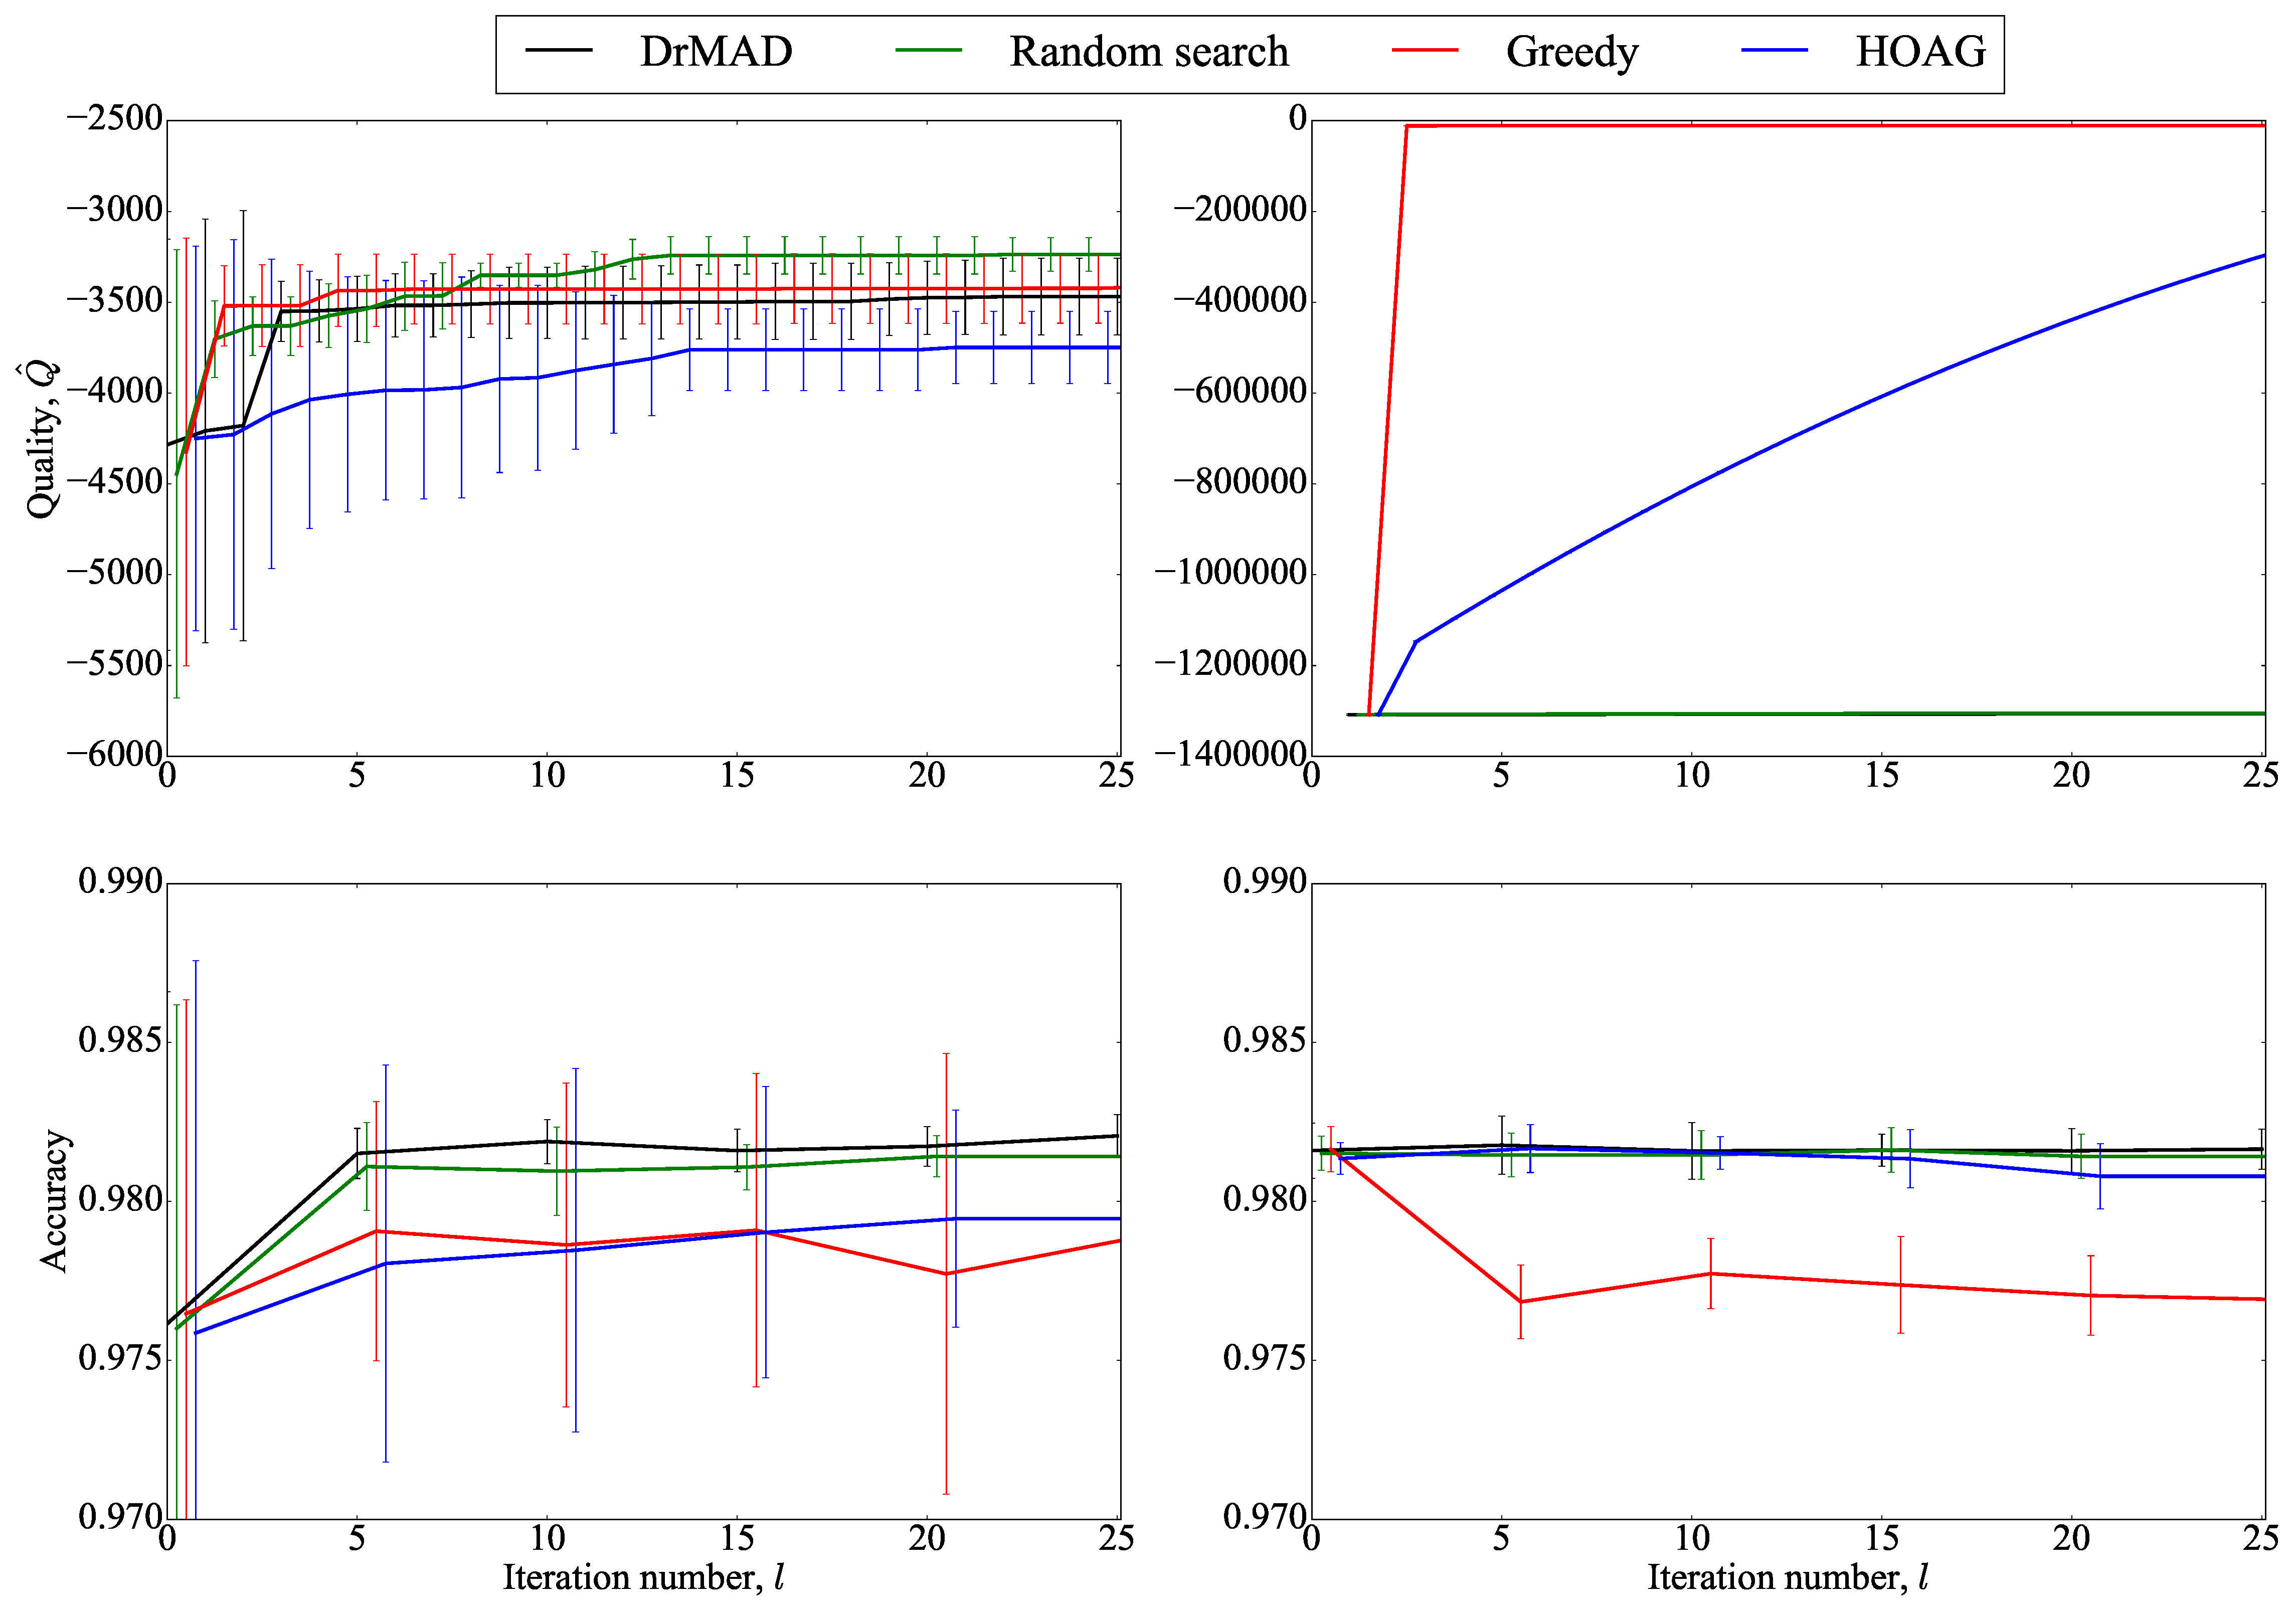
\includegraphics[width=0.7\textwidth]{Fig_mnist.eps}
\end{figure}
\end{frame}

\begin{frame}{Эксперименты: MNIST}
Добавление гауссового шума $\mathcal{N}(\mathbf{0},\sigma^2\mathbf{I})$:
\setlength{\columnsep}{10pt}
\begin{multicols}{4}
\begin{figure}[h]
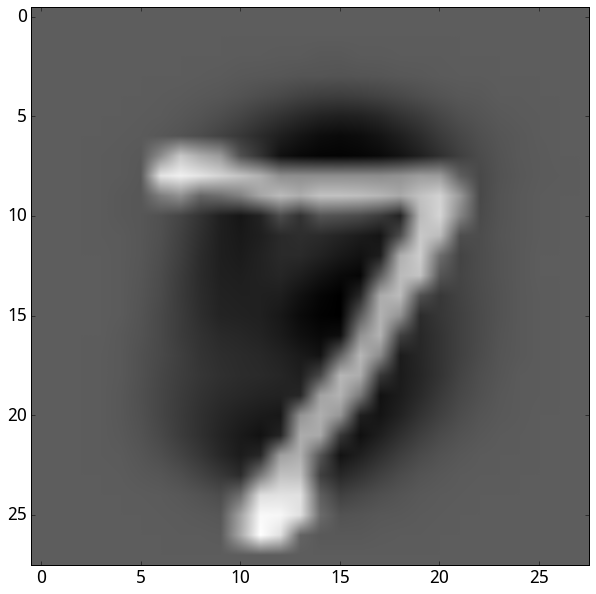
\includegraphics[width=0.10\textwidth]{./mnist0.png}
\caption*{Без шума}
\end{figure}

\begin{figure}[h]
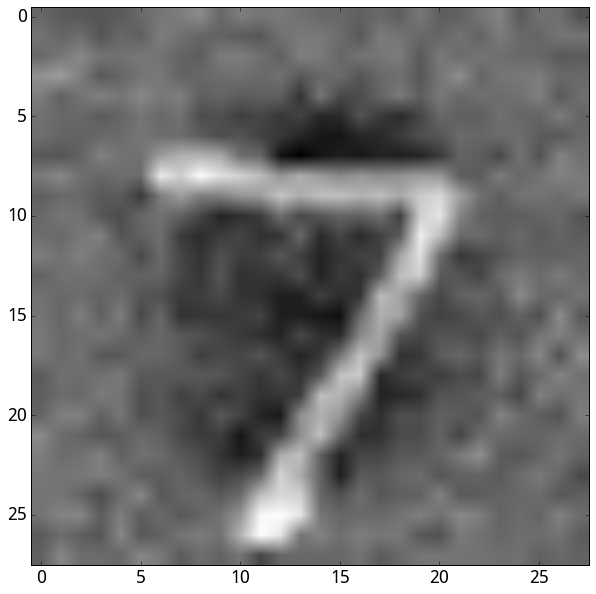
\includegraphics[width=0.08\textwidth]{./mnist10.png}
\caption*{$\sigma=0.1$}
\end{figure}

\begin{figure}[h]
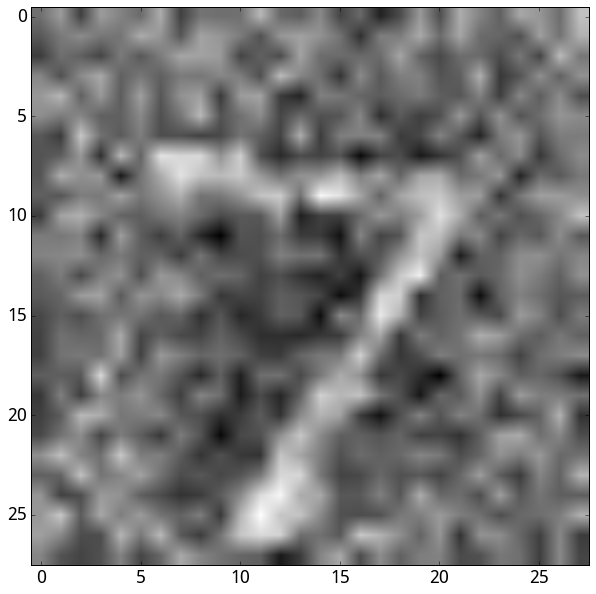
\includegraphics[width=0.08\textwidth]{./mnist25.png}
\caption*{$\sigma=0.25$}
\end{figure}

\begin{figure}[h]
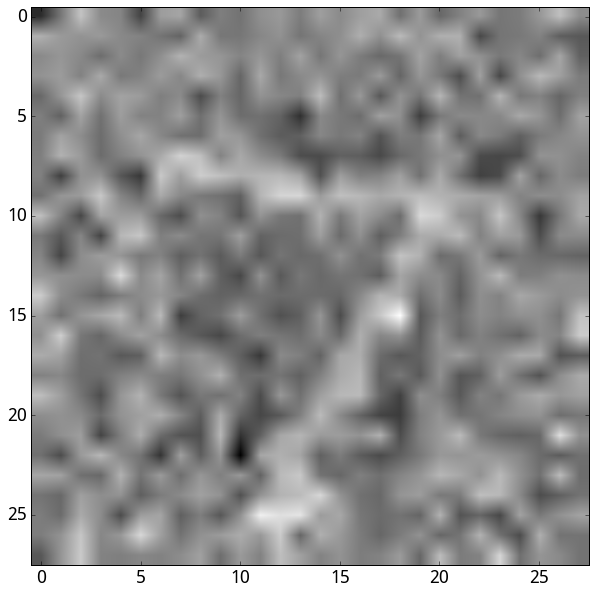
\includegraphics[width=0.08\textwidth]{./mnist50.png}
\caption*{$\sigma=0.5$}
\end{figure}
\end{multicols}
\begin{center}
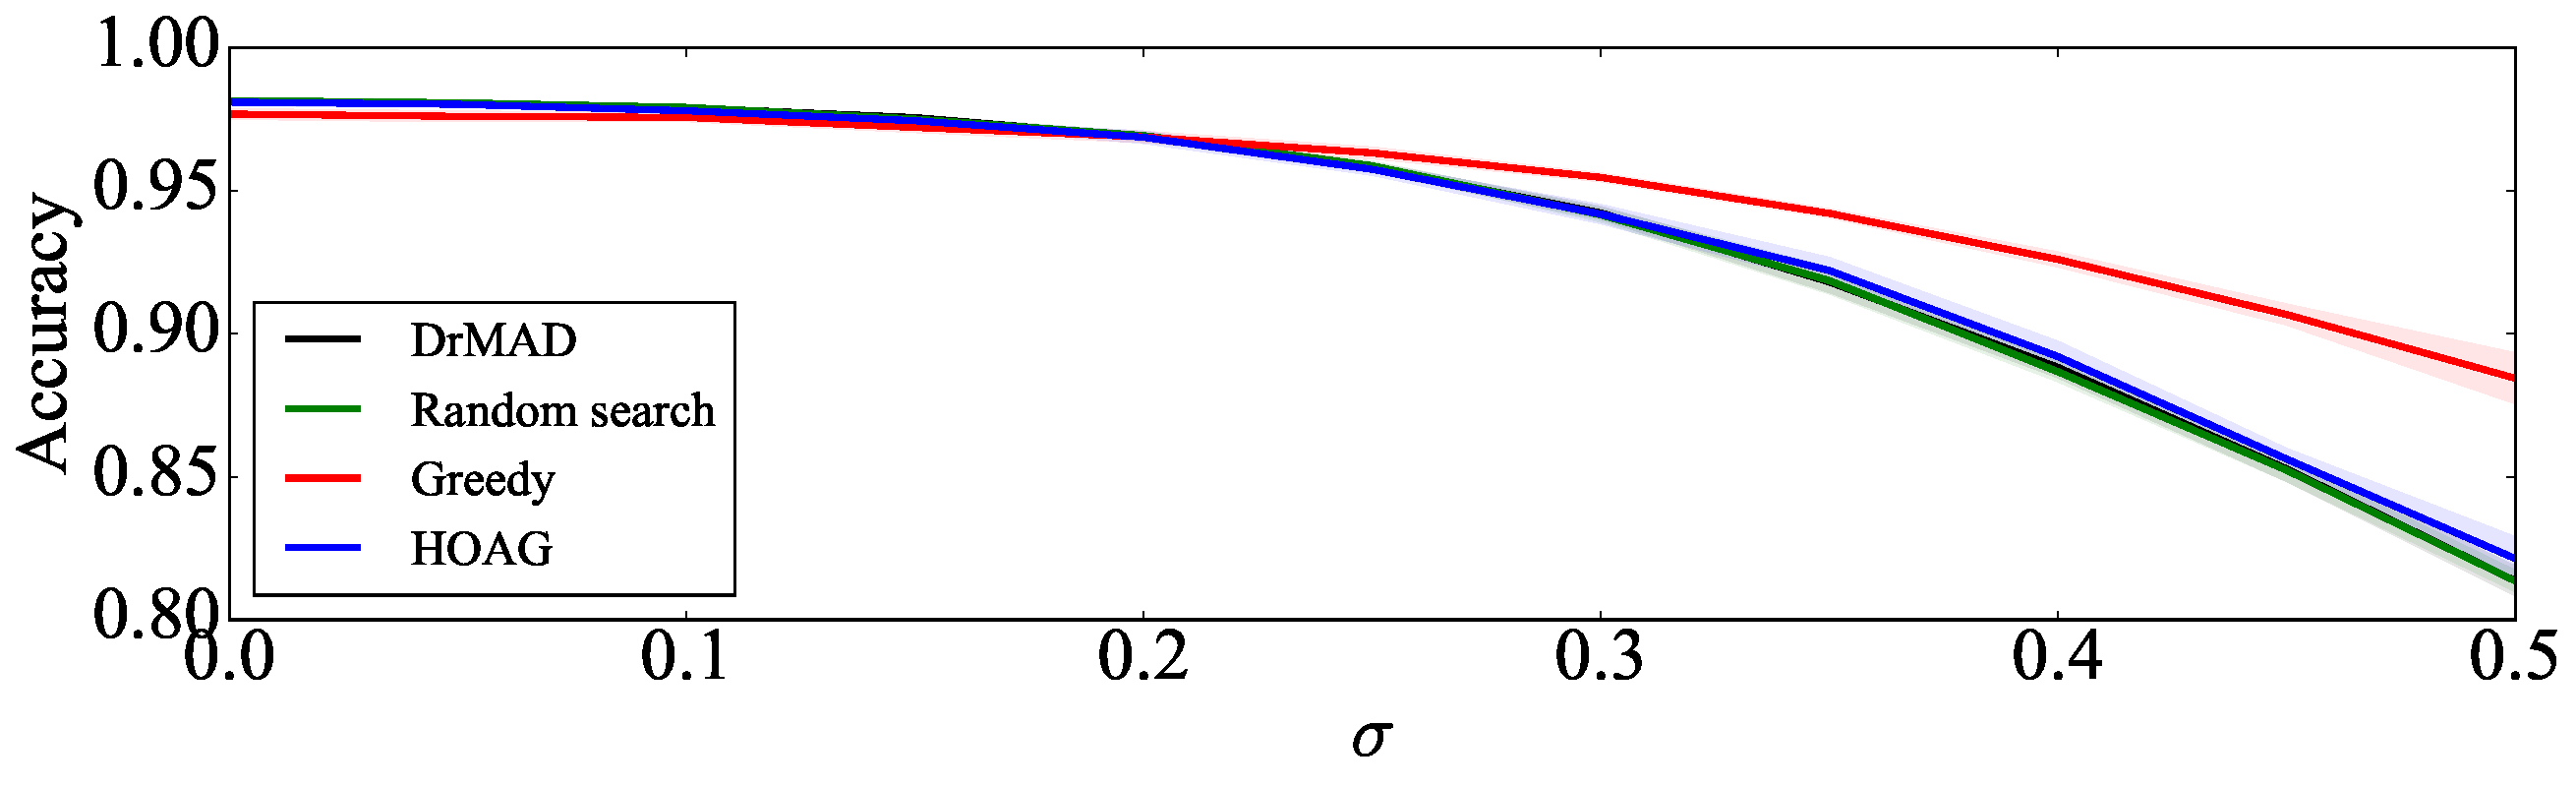
\includegraphics[width=0.85\textwidth]{Fig_noise.pdf}
\end{center}
\end{frame}

\begin{frame}
\frametitle{Используемые материалы}
\begin{enumerate}
\item David J. C. MacKay, Information Theory, Inference \& Learning Algorithms, 2003
\item Christopher Bishop, Pattern Recognition and Machine Learning, 2006
\item  Dougal Maclaurin et. al, Gradient-based Hyperparameter Optimization through Reversible Learning, 2015
\item Jelena Luketina et. al, Scalable Gradient-Based Tuning of
Continuous Regularization Hyperparameters, 2016
\item Jie Fu et. al, DrMAD: Distilling Reverse-Mode Automatic Differentiation for Optimizing
Hyperparameters of Deep Neural Networks, 2016
\item Fabian Pedregosa, Hyperparameter optimization with approximate gradient, 2016
\item Bobak Shahriari et. al,  Taking the Human Out of the Loop:
A Review of Bayesian Optimization, 2016
\end{enumerate}
\end{frame}


\end{document}

